\documentclass{jsarticle}
\usepackage[dvipdfmx]{graphicx}
\usepackage{Here}
\begin{document}

\title{計算機科学実験2ソフトウェア報告書2}
\author{平成30年入学\\1029300562\\新山公太(にいやまこうた)}
\maketitle

\section{課題3}
\subsection{現象の観察}
下の図1のように、課題2で作ったエージェントは敵をよけることができずに3回ぶつかってやられてしまう。
	\begin{figure}[H]
	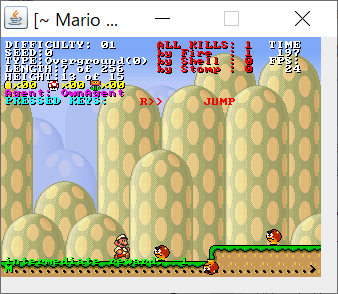
\includegraphics{MainTask3_failed.png}
	\caption{課題2のエージェントでは敵をよけられない}
	\end{figure}
	
\subsection{現象の解析}
課題2で作ったエージェントには敵を発見して避けるという機能を実装していなかったので、こうなってしまうことはわかっていた。解決策としては敵を見つけたときにジャンプするというアクションを実装すれば良いと思われるが、素朴に目の前に敵がいるときにジャンプするという機能だけを疾走してもうまくいかないと思われる。なぜならばジャンプした後に敵とぶつかる場合については、この処理では対応できない。この事態を避けるためには、敵が目の前にいるときにはファイヤーボールで敵を攻撃して倒してしまえばよいだろう。もしファイヤーボールを撃てる状態でなければ、敵にぶつからないようにマリオの軌道を変えればよいだろう。具体的には目の前に敵がいる状況について、敵とある程度の距離がある場合はファイヤーボールを放ちつつ、至近距離に敵がいる場合についてはジャンプで避けるという方針になる。この際に気を付けなければならないことは敵が自分より高い位置から降ってくる場合について対処することである。
\subsection{実装}
\subsubsection{作ったメソッド}

\begin{description}
	\item [isObstacle(int r, int c) :] 
	このメソッドはマリオの移動を制限する物体がマリオの位置を(9,9)とした座標で(9-r,9+c)にある時にtrueを返すメソッドである。

	\item [noObstacle(int r, int c) :] 
	このメソッドはマリオの位置を(9,9)とした座標において(9-r,9+c)に物体がないときにtrueを返すメソッドである。
	これは次のisHole()メソッドを書くために作った。

	\item [isHole(int fr) :]
	このメソッドはマリオの前方frマス目に落とし穴があるかどうかを判定するメソッドである。

	\item [isEnemy(int x, int y) :]
	このメソッドはマリオの位置を(9,9)とした座標において、(9+x)の位置をマリオの目線からyマス上までみてそこに敵がいればtrueを返すメソッドである。

	\item [falling(float y1, float y2) :]
	このメソッドはマリオの詳細な位置情報を用いて、マリオが落下しているかどうかを判定するために作ったメソッドである。

\end{description}

\subsection{作ったルール}
javaプログラムでは変数への代入は上の行から順番に行われるために、getAction()メソッドの中で変数に複数回の代入が行われると、一番下の行で代入された値が格納されてキーの情報が呼び出される。このために優先度の低い順にルールを記述していけばよい。

\subsubsection{jump}
デフォルトの状態としてジャンプボタンは押さない。もしマリオの前に障害物があれば、地上にいないかジャンプ可能であるときジャンプボタンを押し、そうでなければジャンプボタンを押さない。もしマリオの頭の上2マスに敵がいる場合ジャンプボタンは押さない。マリオの1マス前または2マス前のそれぞれに関して、マリオの頭の上の3マスに敵がいるならば、地上にいないかジャンプ可能であるときジャンプボタンを押し、そうでなければジャンプボタンを押さない。マリオの1マス前に足場がなければ、マリオが地上にいないかジャンプ可能であるときジャンプボタンを押し、そうでないときはジャンプボタンは押さない。

\subsubsection{dash}
ダッシュボタンはデフォルトでは押されない。マリオの周りに敵がいる時といない時について分けて考える。いるときは、マリオがファイヤマリオでかつ、敵がマリオの周りにいるときにダッシュボタンを押し、trueSpeedCounterをインクリメントする。そうでないときはダッシュボタンは押さずtrueSpeedCounterに0を代入する。
周りに敵がいないとき、trueSpeedCounterが0でマリオがファイヤマリオならダッシュボタンをおして、trueSpeedCounterをインクリメントする。
これはファイヤボールを乱発して、できるだけ多くの敵を倒せば危険を回避しやすくなることを考えたルールである。また、敵が周りにいる、いないに関係なく目の前か自分のいる位置の下に障害物がなければダッシュボタンを押しておく。
\subsubsection{left}
左ボタンはデフォルトでは押されない。マリオの頭よりも上に敵がいるとき、上から敵が降ってくるということで危ないので左ボタンを押して危険を回避する。しかしこの方法では崖の下にマリオがいて、崖の上に土管に潜んでいるパックンフラワーにも反応して動けなくなってしまうことがあったので、それを回避するためにその状況においては左ボタンを押さないようにした。また他に危ない状況として、落とし穴を超えている途中に落下し始めたら左に戻って安全を確保するために左ボタンを押すようにした。
\subsubsection{right}
右ボタンはデフォルトで押されている。敵がマリオの下にいてマリオがジャンプ中ならば敵を踏み潰すために右ボタンを押さないようにする。また、敵がマリオの頭上から降ってくる状況については危険を回避するために右ボタンを押さないようにする。これについても左ボタンの時と同じように土管の中に潜んでいるパックンフラワーに対処するための条件をつけて、その時は右ボタンを押すようにした。また落とし穴が目の前にあって落下中の時についても左ボタンの時と同じ考え方で、危ないので左に戻るために右ボタンは押さないようにする。
\subsection{検証}
下図に示すように今回作ったエージェントの最大の工夫である上から落ちてくる敵への対処はある程度うまく機能していることがわかる。そのおかげで、この面に関しては一度もダメージを受けることなくクリアすることができた。シード値を変えてどのくらいの割合でクリアできるかを調べてみると大体70\%くらいの割合でクリアすることができ、クリアできないケースに関しては落下して敵の目の前に落ちてしまう、パックンフラワーの時と同じように埋まっている敵に反応してしまうなどが原因であった。敵の目の前に落ちてしまうケースは、敵の位置をマス目で判定しており大雑把であるので難しかった。敵の位置をfloat型で取得するメソッドをあとから見つけたので、これは改良できそうである。地面に埋まっている敵に関しては障害物があるかどうかを判定するメソッドと敵がいるかどうかを判定するメソッドを一緒に使えば、対処できるように思われる。後期の終わりまでに時間があれば改良したいと思う。

\begin{figure}[H]
	\begin{tabular}{c}
	\begin{minipage}{0.50\hsize}
		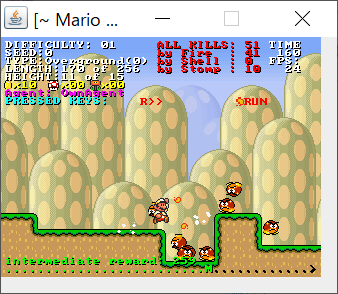
\includegraphics{avoid1.png}
		\caption{落下してくる敵をよける1}
	\end{minipage}
	\begin{minipage}{0.50\hsize}
		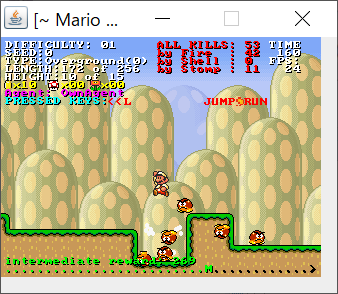
\includegraphics{avoid2.png}
		\caption{落下してくる敵をよける2}
	\end{minipage}
\\
	\begin{minipage}{0.06\hsize}
       	 \vspace{10mm}
      \end{minipage}
\\

	\begin{minipage}{0.50\hsize}
		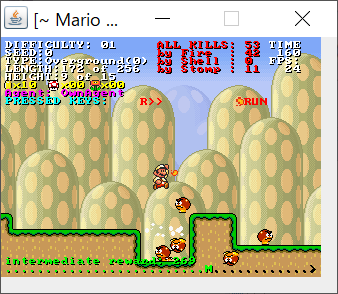
\includegraphics{avoid3.png}
		\caption{落下してくる敵をよける3}
	\end{minipage}
	\begin{minipage}{0.50\hsize}
		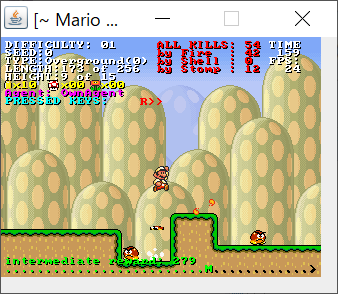
\includegraphics{avoid4.png}
		\caption{落下してくる敵をよける4}
	\end{minipage}
	\end{tabular}
\end{figure}

\section{課題4}
\subsection{基本課題}
この課題で設定されているステージには下図のように高い崖がありステージの片側がふさがっている。この課題はルールベースではなく遺伝アルゴリズムを用いてエージェントを作成した。このエージェントは$2^{16}$通りの状態を管理している。つまり各ビットに対して対応する条件が定められており、その条件を満たすときはそのビットは1満たさないのなら、0が格納されている。4-1を学習させたエージェントに格納する条件はあまり上手に作られたものではなく、同じ条件を二回判定していたりするがそれでもゴールしてくれる個体が生まれた。
\begin{figure}[H]
	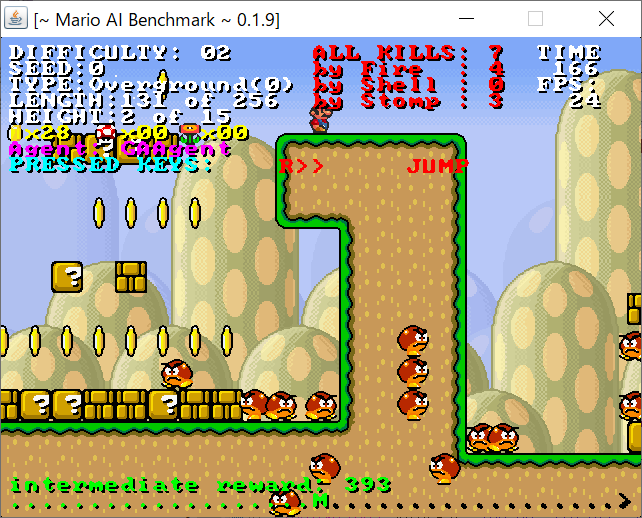
\includegraphics{wall.png}
	\caption{高い壁}
\end{figure}
\subsubsection{判定する状態}
\begin{itemize}
	\item{敵が1マス前の頭上3マスまでにいるか}
	\item{敵が1マス後ろの頭上3マスまでにいるか}
	\item{物体が1マス前の頭上3マス上までにあるか}
	\item{物体が1マス後ろの頭上3マス目までにあるか}
	\item{マリオの真下に足場があるか}
	\item{物体が2マス前の頭上3マス上までにあるか}
	\item{1マス前に落とし穴があるか}
	\item{マリオの頭上3マスまでに物体があるか}
	\item{敵が2マス前の頭上3マスまでにいるか}
	\item{敵が1マス前の3マス下までにいるか}
	\item{画面内に壁があるか}
	\item{マリオが右に進んでいるか}
	\item{マリオが地上にいるか}
	\item{マリオがジャンプ可能か}
\end{itemize}
\subsubsection{補足}
扱える状態を無駄にしている部分が多かったので4-3と同じ条件で学習したところ、そちらでもクリアできる個体が生まれた。
\subsection{発展課題}
\subsubsection{MainTask4\_2}
4-2でも4-1と同じ条件で学習させるとクリアしてくれる個体が生まれた。結局は、実際に重要な状態だけから行動が決められるわけではないので、持たせている条件が頻繁に重複しなければ過学習することでそのステージに関してはうまい操作方法を見つけてくれるのではないだろうか。実際に4-1のエージェントで4-2をプレイさせてみたところ、優秀とは言えない成績だった。
また、途中でスモールマリオの状態でないと通ることのできない隙間があり、そこを通ってクリアしているためにわざと敵とぶつかっていることが確認できた。以下の図に示すような、キラー砲台と天井の間はファイヤーマリオもしくは通常状態のマリオでは通り抜けることができない。
\begin{figure}[H]
	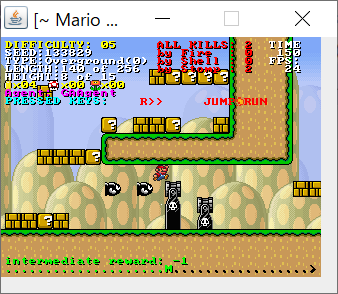
\includegraphics{narrow1.png}
	\caption{狭い通り道}
\end{figure}
\subsubsection{MainTask4\_3}
4-3については条件のうち重複しているものがあることに気が付いたので、修正を加えて学習させてみた。しかし現段階ではこの面をクリアする個体は生まれなかった。この面は越えなければならない難所が多く、遺伝アルゴリズムで何世代も学習させても途中のどこかで詰まってしまって、なかなか進んでくれなかった。対処法として思いついたのが、コースを複数の区間に分割して各区間において遺伝アルゴリズムで学習させるというものであるが、時間がなくこのレポートの提出までには実装できなかった。後期の実験が終わるまで再提出が認められていたのでそれまでに実行したい。
\subparagraph{判定する状態}
4-3では判定する状態を一つ増やして17個とした。(実際には4-1,4-2では二つの状態をつぶしているので新しく判定できる条件は3つ増えている。つまり元の条件の$2^3$倍の状態を持つことができる.)
\begin{itemize}
	\item{敵が1マス前の頭上3マスまでににいるか}
	\item{敵が1マス前の下3マスまでにいるか}
	\item{敵が1マス後ろの3マス頭上にいるか}
	\item{自分と同じ高さに敵がいるか}
	\item{自分の1マス下の高さに敵がいるか}
	\item{自分の1マス上の高さに敵がいるか}
	\item{目の前に落とし穴があるか}
	\item{自分の下の2マス目までに敵がいるか}
	\item{自分の下に足場があるか}
	\item{物体が1マス前の頭上3マスまでにあるか}
	\item{物体が1マス前の下3マスまでにあるか}
	\item{物体が1マス後ろの頭上3マスまでにあるか}
	\item{物体が1マス後ろの下3マスまでにあるか}
	\item{物体が頭上2マス目までにあるか}
	\item{敵が自分の右側の近くにいるか}
	\item{マリオが地面にいるか}
	\item{マリオがジャンプ可能か}
\end{itemize}

\begin{figure}
	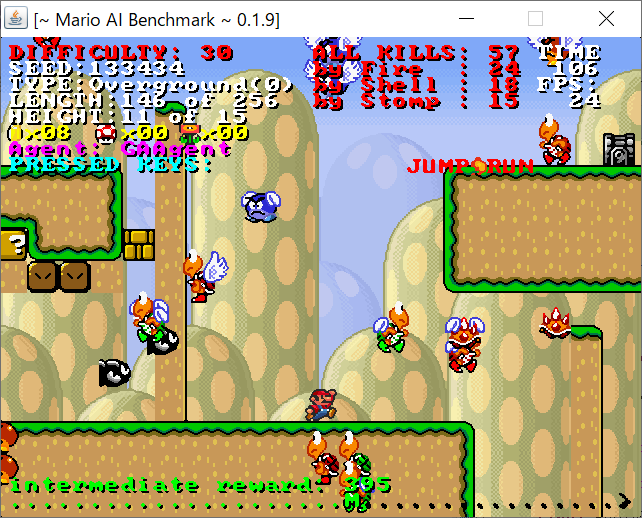
\includegraphics{deadpoint.png}
	\caption{突破できないところ}
\end{figure}

この辺りで、敵を踏みつけて上の経路にいければ攻略難易度が少し下がるのではないかと思う。評価関数において踏みつけによって敵を倒した時のスコアを高めに設定してやるとうまくいくかもしれない。
他にもいくつか打開策の候補は思いついたのだが、提出期限の関係でとりあえずこの段階でレポートとしてまとめた。

\subsubsection{以後の攻略の方針}
4-3をクリアできていないのは、難所が多くうまい状態の持たせ方ができていないのが一番の原因であると考察している。ステージの状態の持たせ方を工夫することで、解の数が増えると予想される。極論をいえば目の前に敵がいるかどうかだけを判定して2通りの状態しか持っていない場合、行動も必然的に2通りで、スタートからゴールまでの各行動においていずれかの行動のみでクリアするのは現実的に考えて無理である。ここまで極端な状況でないにしろ、現状学習があまりうまく進んでいない以上持たせる状態について問題がないとは言えない。しかし、配列に格納できる整数の大きさの制限から、単に状態を増やせばよいというわけでもない。

そこで思いついたのが最初から2種類の遺伝子を持たせておき、前半と後半で遺伝子を使い分ける方法である。こうすれば前半部と後半部で同じ状態を表すときにも別の行動を取ることができる。しかし、この方法では後半の遺伝子が完ぺきという場合であっても、前半の遺伝子が劣っているとき後半の遺伝子の評価は低くなってしまうという欠点がある。これが大きな影響を及ぼすかはわからないので、結局のところ試してみないとわからないということにはなる。

別の方法として、モンテカルロ法による攻略も試す価値はあるだろう。遺伝アルゴリズムの時と同じように任意の条件をbitで管理して状態として持たせれば、いいだろう。

その他にも、あくまでも遺伝アルゴリズムで押し切るならば、難所に差し掛かった時のみ、ルールベースでうまいこと難所を回避するように条件を作ってやればよいと思われる。


\end{document}